\subsubsubsubsection{Bike lane stretch}
\begin{figure}[h]
\centering
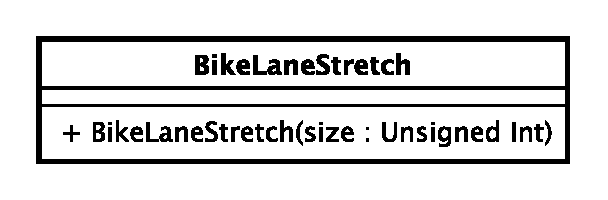
\includegraphics[scale=0.6,keepaspectratio]{images/solution/app/backend/bike_lane_stretch.eps}
\caption{\pReactiveComponentStretch::BikeLaneStretch}
\label{fig:sd-app-bike_lane_stretch}
\end{figure}
\FloatBarrier
\begin{itemize}
  \item \textbf{\descr} \\
    It represents a bike lane stretch entity. It is a protected object. Only bycicles 
can tread this kind of stretch.
  \item \textbf{\ops}
  \begin{itemize}
    \item[+] \texttt{BikeLaneStretch(size : Unsigned Int)} \\
        Creates a bike lane stretch object with a specific size.
  \end{itemize}
\end{itemize}
